\scanpage{357}
\uline{Th Eilenberg-Zilber-Cartier}\hfill EZ 1

$X_{**}$ un \deleted{groupe}\inserted{objet} abelien bisimplical $(\qquad)$.
\deleted{\[
\unsure{N:\mathrm{Ab}(\text{bisimpl.})\longrightarrow A(}
\]}
\diagram{\begin{tikzcd}
N:A_{**}\arrow[r,"\text{eq de cat}","\sim"'] & A_{\bullet\bullet}\\
\widetilde{\phantom{X}}:A_{**}\arrow[r] & A_{\bullet\bullet}\\
\Delta:A_{**}\arrow[r] & A_*\\
\int:A_{\bullet\bullet}\arrow[r] & A_\bullet
\end{tikzcd}}
\margin{(complexe associé}
\margin{\diagram{\begin{tikzcd}
N:A_*\arrow[r] & A_\bullet\\
\widetilde{\phantom{X}}:A_*\arrow[r]&A_\bullet\\
N\arrow[r,hook]&\widetilde{(\ )}\quad\text{q ism}\\
&D(\ )\arrow[u]\quad\text{degen homot triv}
\end{tikzcd}}}

$\exists$ des \deleted{quasi-iso naturels}\inserted{morphismes} fonctoriels,
\diagram{\begin{tikzcd}
\int N\arrow[r,shift right,"\varphi"'] &N\Delta\arrow[l,shift right,"\psi"']
\end{tikzcd}}
\deleted{$X_{0,0}$}
qui coincident avec les fleches evidents en degré 0.
\figure{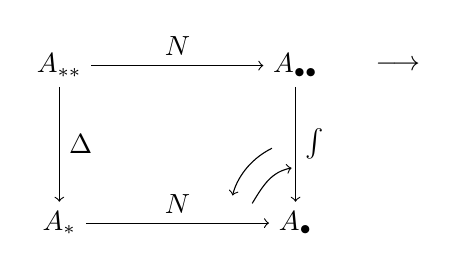
\begin{tikzpicture}
\node(a) at (0,2) {$A_{**}$};\node(b) at (3,2) {$A_{\bullet\bullet}$};
\node(c) at (0,0) {$A_*$};\node(d) at (3,0) {$A_\bullet$};
\draw[->](a)--node[above]{$N$}(b);\draw[->](a)--node[right]{$\Delta$}(c);
\draw[->](b)--node[right]{$\int$}(d);\draw[->](c)--node[above]{$N$}(d);
\node at (4.3,2) {$\deleted{\longrightarrow}$};
\draw[->](2.7,.95) .. controls (2.4,.8) and (2.25,.55) .. (2.2,.35);
\draw[->](2.45,.25) .. controls (2.6,.5) and (2.7,.65) .. (2.95,.7);
\end{tikzpicture}}
\[
\varphi\psi\sim1_{\int N}\qquad\psi\varphi\sim1_{N\Delta}
\]
\deleted{$\unsure{\varphi\psi(X_{**})}$}
\diagram{\begin{tikzcd}
\psi\varphi\int(NX_{**})\arrow[r]&\int NX_{**}\\
\varphi\psi N\Delta X_{**}\arrow[r]&N\Delta X_{**}
\end{tikzcd}}
\[
1-\psi\varphi=dk+kd\qquad1-\varphi\psi=dh+hd
\]
\diagram{\begin{tikzcd}
k:\int NX_{**}\arrow[r,shift left,"+1"]\arrow[r,shift right]&\int NX_{**}\\
h:N\Delta X_{**}\arrow[r,"+1"]&N\Delta X_{**}
\end{tikzcd}}
\figure{\begin{tikzpicture}\draw (0,0)--(4,0);\end{tikzpicture}}
\diagram{\begin{tikzcd}
\int N\arrow[r,shift left,no head,"\psi"]\arrow[d]&N\Delta\arrow[l,shift left,"\varphi"]\arrow[d,no head]\\
\int\widetilde{\phantom X}\arrow[r,shift left,"\widetilde\psi"]&\widetilde{\phantom X}\Delta\arrow[l,shift left,"\widetilde\varphi"]
\end{tikzcd}}
\deleted{$k-h'=$}
\diagram{\begin{tikzcd}
\int\widetilde{\phantom X}\arrow[r,shift right,"\widetilde\varphi"']&\widetilde{\phantom X}(\Delta)\arrow[l,shift right,"\widetilde\psi"']
\end{tikzcd}}
Si $\varphi$ et $\psi$ sont choisis, Pour un autre choix de $k',h'$
\[
k'-k=d\ell+\ell d\qquad h'-h=dm+md
\]
etc\ldots\quad$\ell$ et $m$ fonct

$\exists$ des choix traditionnels: ``application d'Alexander Whitney''
\deleted{EZ 2}
``shuffles''

\tikz[baseline=(m.base)]{\node[inner sep=0](m){cf MacLane};\draw([yshift=-2pt]m.south west)--([yshift=-2pt]m.south east);\draw([yshift=-4pt]m.south west)--([yshift=-4pt]m.south east);\draw([yshift=-6pt]m.south west)--([yshift=-6pt]m.south east);}\quad Homology
\diagram{\begin{tikzcd}
(\int\widetilde X_{**})_n=\displaystyle\bigoplus_{i+j=n}X_{(i)(j)}\arrow[r,"\text{shuffles}"]&\widetilde X_{(n,n)}\\
x_{ij}\arrow[r]&\deleted{\unsure{\sum(-1)s_\alpha s'_\beta(}}\quad x_{i+j,i+j}
\end{tikzcd}}
$(i,j)$-shuffle
\diagram{\begin{tikzcd}
(1\quad\ldots,\overset{\substack{n\\\Vert}}{i+j})\arrow[d,no head]&{}\\
s(1)\quad\ldots\quad\underbrace{s(i)}\quad\underbrace{s(i+j)}&{}
\end{tikzcd}}
\[
x_{i1}\qquad x_{i+1,i+1}
\]
\[
\sum_{0\le\alpha\le i}\unsure{(-1)_{\alpha}|(-1)^\alpha} s'_0s'_1\ldots
\overset{\deleted{\wedge}}{s_\alpha}\ldots s'_i\,x_{i1}
\]
\margin{signe$(\sigma)$}
\[
\sum_{\substack{\text{sur tout }\sigma\in\Sigma_n\\
\text{t.q. }\sigma(\alpha)<\sigma(\beta)\\
\alpha<\beta\le i\ \text{ou}\ \deleted{i<}\ i<\alpha<\beta\le n}}
\underbrace{s_{\sigma(i+1)}\ldots s_{\sigma(i+j)}}\,
\underbrace{s'_{\sigma(1)}\ldots s'_{\sigma(i)}}
\]
$\unsure{\sigma\Box|\sigma\in}$
\figure{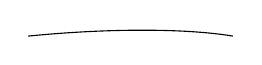
\begin{tikzpicture}\draw (0,0) .. controls (1,.1) and (2,.1) .. (2.6,0);\end{tikzpicture}}
\margin{Shuffles}
\figure{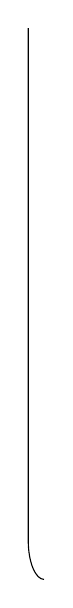
\begin{tikzpicture}
\draw (0,0)--(0,-6.5) .. controls (0,-6.8) and (.1,-7) .. (.2,-7);
\end{tikzpicture}}
\[
A\qquad\overline B(A)
\]
\figure{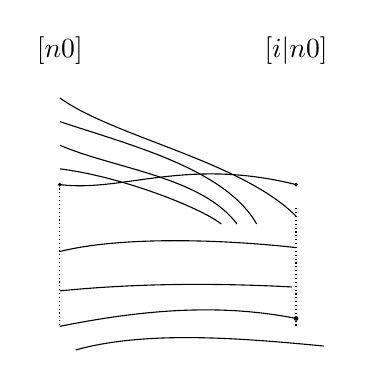
\begin{tikzpicture}[x=1cm,y=1cm]
\node at (0,2.7) {$[n\deleted{\unsure{0}}]$};
\node at (3,2.7) {$[\unsure{i|n}\deleted{\unsure{0}}]$};
\draw (0,2.1) .. controls (.7,1.6) and (2.3,1.3) .. (3,.6);
\draw (0,1.8) .. controls (.9,1.5) and (2.1,1.2) .. (2.5,.5);
\draw (0,1.5) .. controls (.7,1.2) and (1.8,1.1) .. (2.25,.5);
\draw (0,1.2) .. controls (.8,1.1) and (1.8,.7) .. (2.05,.5);
\draw (0,1) .. controls (.8,.9) and (1.6,1.35) .. (3,1);
\draw (0,.15) .. controls (.8,.35) and (2.1,.3) .. (3,.2);
\draw (0,-.35) .. controls (1,-.25) and (2,-.25) .. (2.95,-.3);
\draw[densely dotted] (0,1)--(0,-.8);
\draw[densely dotted] (3,.7)--(3,-.8);
\draw (0,-.8) .. controls (1,-.6) and (2,-.5) .. (3,-.7);
\draw (.2,-1.1) .. controls (1.1,-.85) and (2.3,-.95) .. (3.35,-1.05);
\fill (0,1) circle (.025);\fill (3,1) circle (.025);\fill (3,-.7) circle (.03);
\end{tikzpicture}}

\uuline{Alexander-Whitney}
\diagram{\begin{tikzcd}
\widehat X_{n,n}\arrow[r]&\bigoplus X_{ij}\\
x_{n,n}\arrow[r]&\displaystyle\sum_{i=0}^n(-1)^i d_0^{n-i}\widehat d^{\,i}x_{n,n}
\end{tikzcd}}
\diagram{\begin{tikzcd}[column sep=small]
\underset{f}{\underbrace{C^i(X,A)}}\otimes\underset{g}{\underbrace{C^j(X,B)}}\arrow[r,Rightarrow]&C^{i+j}(X\times X,A\otimes B)\arrow[r,bend right=15]&C^{i+j}(X,A\otimes B\\
ZX\otimes ZX&Z(X\times X)\arrow[l,Rightarrow]\arrow[r,bend right=20,no head]&{}
\end{tikzcd}}
$\widehat d$ signifie le dernier op face

$d'$ seconde op simpl.
\[
\widehat d^{\prime i}=\underbrace{d^{\prime n}d^{\prime n-1}\ldots d^{\prime n-i+1}}
\]
\[
\mathrm{E\!-\!Z\!-\!C}\Rightarrow\mathrm{E\!-\!Z}
\]
Cup-produit
\[
\left\{\begin{aligned}
h(x_1,\ldots,x_{n+1})\\
{}=\sum(-1)f(x_1\ldots x_i)g(x_{i+1},\ldots x_n)
\end{aligned}\right\}
\]
\uline{associatif}\quad(non-commutatif mais comm. à homotopie près)
\[
\Rightarrow H^*(X,R)\quad\text{est anticom.}
\]
\mspage{358}
